\documentclass{article}
\usepackage[margin=1in]{geometry}
\usepackage{tikz}
\usepackage{amsmath}
\usepackage{amssymb}
\usepackage{multicol}
\usepackage{import}

\import{../}{labflowchart.sty}

\begin{document}
\title{Lab 0 - Rubber Stoppers}
\author{Aaron Huang}
\date{February 12, 2026}
\maketitle
\section{Purpose}
\begin{enumerate}
    \item To determine the density of two sizes of rubber stoppers
    \item To write up a complete lab report using proper format
\end{enumerate}
\section{Introduction}

Density was defined as a physical property that described the relationship between the mass of a material and its volume, calculated using  $\rho = \frac{m}{V}$. In this formula the density was represented by $\rho$, the mass was represented by $m$, and the volume was represented by $V$.

Water-displacement and mass measurements were used to determine the volumes and densities of two rubber stoppers. The smaller stopper volume was determined by graduated-cylinder displacement; the larger stopper volume was determined by measuring the change in mass of a watch glass after overflow collection. Calculations were performed using measured masses and displaced-volume values to obtain densities.

There were no special safety considerations for this experiment. 


\section{Materials}
\begin{itemize}
    \item Graduated cylinder (200 mL)
    \item Two rubber stoppers (small \& large)
    \item Beaker (50 mL)
    \item Watch glass
    \item Water
    \item Mass scale
    \item Dropper
\end{itemize}
\newpage
\subsection{Apparatus}
    \vspace{0.125 in}
    \begin{figure}[h]
        \centering
        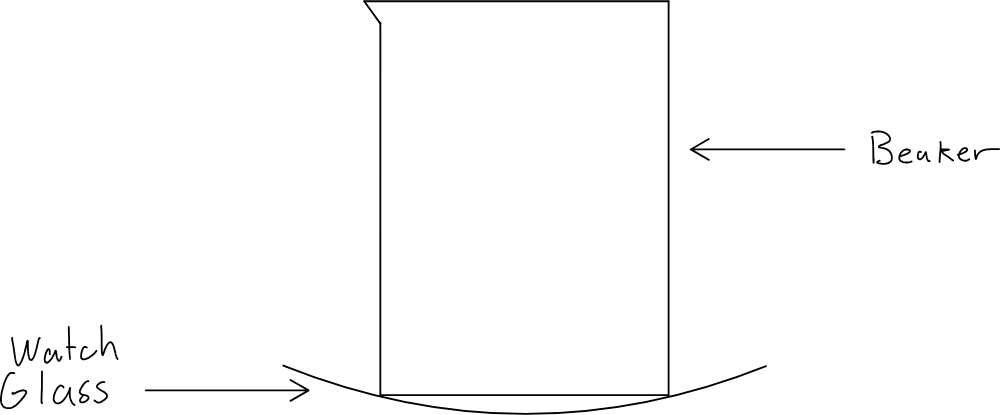
\includegraphics[width=0.75\linewidth]{Images/Figure 3.1.1 - Apparatus.png}
        \caption{Apparatus used for part two of the experiment}
        \label{fig:apparatus}
    \end{figure}
\section{Procedure}
% part 1
% \subsection{Part 1: Density of Small Rubber Stopper}
% \begin{procedureflowchart}
%     % --- Step 1: Mass of Small Rubber Stopper ---
%     \lstep{Mass Scale}
%     \rstep{Mass of the small rubber stopper was measured}

%     % --- Step 2: Initial Water Level ---
%     \lstep{Graduated Cylinder} 
%     \rstep{Graduated cylinder was filled to an intermediate level}
%     \rstep{Initial water level was recorded}

%     % --- Step 3: Final Water Level ---
%     \lstep{Small stopper}
%     \rstep{Small rubber stopper was lowered into the cylinder}
%     \rstep{Water was stirred to remove trapped bubbles}
%     \rstep{Final water level was recorded}
% \end{procedureflowchart}
% \newpage
% \subsection{Part 2: Density of Large Rubber Stopper}

\begin{procedureflowchart}
    % --- Step 1: Mass of Large Rubber Stopper ---
    \lstep{Mass Scale}
    \rstep{Mass of the large rubber stopper was measured and recorded}
    \rstep{Initial mass of the watch glass was measured and recorded}

    % --- Step 2: Initial Water Level in Beaker ---
    \lstep{Beaker (50 mL)}
    \rstep{Beaker was filled leaving handling clearance}
    \rstep{Beaker was placed on the watch glass to collect overflow}
    \lstep{Dropper}
    \rstep{Water was added using a dropper until beaker was full}
    \lstep{Large Stopper}
    \rstep{Stopper was slowly and carefully lowered into the beaker}
    \lstep{Dropper}
    \rstep{Excess water was removed to avoid spillage}
    \lstep{Mass Scale}
    \rstep{Final mass of the watch glass with collected water was measured and recorded}
\end{procedureflowchart}

\section{Observations}
\begin{table}[ht!]
    \centering
    \caption{Observations of Rubber Stoppers — Small}
    \label{tab:observations-small}
    \vspace{0.125 in}
    \begin{tabular}{|c|c|c|}
        \hline
        \textbf{Mass (g)} & \textbf{Initial Measurement (mL)} & \textbf{Final Measurement (mL)} \\
        \hline
        4.33 & 15.1 & 16.8 \\
        \hline
    \end{tabular}

\end{table}

\vspace{0.2in}

\begin{table}[ht!]
    \centering
    \caption{Observations of Rubber Stoppers — Large}
    \label{tab:observations-large}
    \vspace{0.125 in}
    \begin{tabular}{|c|c|c|}
        \hline
        \textbf{Mass (g)} & \textbf{Initial Measurement (g)} & \textbf{Final Measurement (g)} \\
        \hline
        24.25 & 25.59 & 41.07 \\
        \hline
    \end{tabular}

\end{table}

\section{Analysis}
%\subsection{Density of Small Rubber Stopper}
\noindent
\begin{minipage}[t]{0.45\textwidth}
    \begin{align*}
        \text{Volume} &= \text{Final} - \text{Initial} \\
        &= 16.8 \text{ mL} - 15.1 \text{ mL} \\
        &= 1.7 \text{ mL} \\
        &= 1.7 \text{ cm}^3
    \end{align*}
\end{minipage}
\hfill
\begin{minipage}[t]{0.45\textwidth}
    \begin{align*}
        \text{Density} &= \frac{\text{Mass}}{\text{Volume}} \\
        &= \frac{4.33 \text{ g}}{1.7 \text{ cm}^3} \\
        &\approx 2.6 \text{ g/cm}^3
    \end{align*}
\end{minipage}\\

The density of water was assumed to be 1 g/mL, the calculation for the large stopper was similar.
% \subsection{Density of Large Rubber Stopper}
% \noindent
% \begin{minipage}[t]{0.45\textwidth}
%     \begin{align*}
%         \text{Volume} &= (\text{Final Mass} - \text{Initial Mass}) \times 1 \text{ g/mL}\\
%         &= 41.07 \text{ g} - 25.59 \text{ g} \\
%         &= 15.48 \text{ g} \\
%         &= 15.48 \text{ mL} \\
%         &= 15.48 \text{ cm}^3
%     \end{align*}
% \end{minipage}
% \hfill
% \begin{minipage}[t]{0.45\textwidth}
%     \begin{align*}
%         \text{Density} &= \frac{\text{Mass}}{\text{Volume}} \\
%         &= \frac{24.25 \text{ g}}{15.48 \text{ cm}^3} \\
%         &\approx 1.567 \text{ g/cm}^3\\
%     \end{align*}
% \end{minipage}
% Summary table of results
\begin{table}[h!]
    \centering
    \caption{Summary of Density Results}
    \label{tab:results-summary}
    \vspace{0.125 in}
    \begin{tabular}{|c|c|}
        \hline
        \textbf{Rubber Stopper} & \textbf{Density (g/cm$^3$)} \\
        \hline
        Small & 2.6 \\
        \hline
        Large & 1.567 \\
        \hline
    \end{tabular}
\end{table}

\section{Discussion}
% 1. Assuming the two rubber stoppers were made of the same material, calculate the percentage error for the method from Part 2.  Assume the result from Part 1 was the “correct” answer.

% 2. One application of density determination is the ability to determine % composition of pure materials in a mixture.  Brass is one example.  Brass is made of copper & zinc.  How would the experiment be modified in order to determine the % composition of copper & zinc in brass?

\begin{enumerate}
    \item 
    With data in Table \ref{tab:results-summary}, the percentage error for the method from Part 2 was calculated as follows:
    \begin{align*}
        \text{Percentage Error} &= \left| \frac{\text{Experimental Value} - \text{Theoretical Value}}{\text{Theoretical Value}} \right| \times 100\% \\
        &= \left| \frac{1.567 - 2.6}{2.6} \right| \times 100\% \\
        &\approx 40\%
    \end{align*}
    
    $\therefore$ the percentage error for the method from Part 2 was approximately 40\%.

    The error in the method from Part 2 could be attributed to several factors. One significant source of error was the surface tension of the water, which may have caused the water to cling the bottom of the beaker when it was removed from the watch glass, leading to an underestimation of the volume of water displaced by the large rubber stopper. 
    
    \item 
    % To find the percentage composition of copper and zinc in a brass sample:
    % \begin{enumerate}
    %     \item Take the mass of the brass sample using a mass scale.
    %     \item The volume of the brass sample would be determined using water displacement in a graduated cylinder.
    %     \item The density would be calculated using the formula $\rho = \frac{m}{V}$.
    %     \item The percentage composition of copper and zinc in the brass sample could be determined by using a system of equations with the known densities of pure copper and pure zinc.
    % \end{enumerate}
    To find the percentage composition of copper and zinc in a brass sample, a similar procedure to the one used for the rubber stoppers may be followed. To begin, the mass of the brass sample would be taken using a mass scale. Then the volume of the brass sample would be determined using water displacement in a graduated cylinder. Next, the density would be calculated using the formula $\rho = \frac{m}{V}$. Lastly, using the known densities of pure copper and pure zinc, a system of equations would be used to solve for the percentage composition of copper and zinc in the brass sample.
\end{enumerate}
\section{Conclusion}
The density of the small rubber stopper was approximately 2.6 g/cm$^3$, and the density of the large rubber stopper was approximately 1.567 g/cm$^3$, with a percentage error of 40\%. A lab report was written with proper formatting.
\end{document}